\documentclass[border=5pt]{standalone}
\usepackage{pgfplots}
\pgfplotsset{compat=1.18}
\usepgfplotslibrary{fillbetween}
\begin{document}
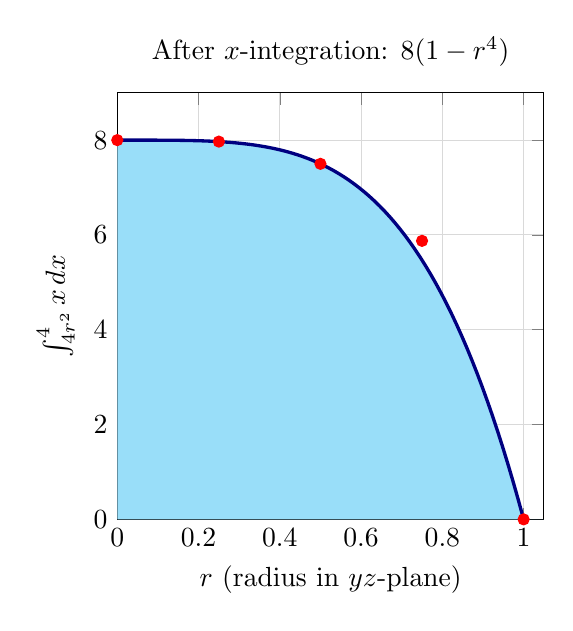
\begin{tikzpicture}
\begin{axis}[
    xlabel={$r$ (radius in $yz$-plane)},
    ylabel={$\int_{4r^2}^{4} x\,dx$},
    xmin=0, xmax=1.05, ymin=0, ymax=9,
    width=7cm, height=7cm,
    title={After $x$-integration: $8(1-r^4)$},
    grid=both, grid style={gray!30}
]
\addplot[name path=curve, blue!50!black, very thick, samples=80, domain=0:1] {8*(1-x^4)};
\path[name path=axis] (0,0) -- (1.05,0);
\addplot[cyan!40] fill between[of=curve and axis];

\addplot[red, only marks, mark=*, mark size=2] coordinates {
    (0.00, 8) (0.25, 7.96875) (0.50, 7.5)
    (0.75, 5.875) (1.00, 0)};
\end{axis}
\end{tikzpicture}
\end{document}